\pdfoutput=1

\documentclass{l4proj}

%
% put any packages here
%
\usepackage{float}
\usepackage[labelfont=bf]{caption}

\usepackage{subfigure}

\usepackage{cleveref}

\setcounter{tocdepth}{3}
\usepackage{graphicx}
\usepackage{algorithmic}
\usepackage[ruled,vlined]{algorithm2e}
\usepackage{url}
\usepackage{alltt}
\urldef{\mailsa}\path|pat@dcs.gla.ac.uk|
\newcommand{\keywords}[1]{\par\addvspace\baselineskip
\noindent\keywordname\enspace\ignorespaces#1}
\newlength{\halftextwidth}
\setlength{\halftextwidth}{0.47\textwidth}

\usepackage{amsopn}
\DeclareMathOperator{\mod}{mod}

\newtheorem{theorem}{Theorem}
\newtheorem{definition}{Definition}


\renewcommand{\figurename}{Fig.}
\Crefformat{figure}{#2Fig.~#1#3}
\Crefmultiformat{figure}{Figs.~#2#1#3}{ and~#2#1#3}{, #2#1#3}{ and~#2#1#3}

\usepackage{listings}
\usepackage{color}

\definecolor{dkgreen}{rgb}{0,0.6,0}
\definecolor{gray}{rgb}{0.5,0.5,0.5}
\definecolor{mauve}{rgb}{0.58,0,0.82}

\lstset{
  %frame=tb,
  language=Java,
  %aboveskip=3mm,
  %belowskip=3mm,
  showstringspaces=false,
  columns=flexible,
  %basicstyle={\small\ttfamily},
  basicstyle=\scriptsize,     % the size of the fonts that are used for the code  
  numbers=left,
  stepnumber=1,
  numberstyle=\small\color{gray},    % the size of the fonts that are used for the line-numbers
  numbersep=10pt,             % how far the line-numbers are from the code
  keywordstyle=\color{blue},
  commentstyle=\color{dkgreen},
  stringstyle=\color{mauve},
  breaklines=true,            % sets automatic line breaking
  breakatwhitespace=false,    % sets if automatic breaks should only happen at whitespace
  showstringspaces=false,     % Don't show underscores as space characters
  %tabsize=4,
  frame=trBL,                 % adds a frame around the code
  frameround=fttt,
  captionpos=b,               % sets the caption-position to bottom
}

\begin{document}

\title{Animating a Sudoku solver}
\author{Gabriel I. Stratan}
\date{November 18, 2015}
\maketitle

\begin{abstract}
Sudoku is a popular puzzle played all over the world. It consists of filling in a 9x9 grid such that every row, column and 3x3 sub-grids have different digits from 1 to 9. Solving the puzzle will make use of the all-different algorithm from Constraint Programming for which an implementation will be provided. Finally, the program will animate all the steps done by the algorithm.
\end{abstract}

\educationalconsent
%
%NOTE: if you include the educationalconsent (above) and your project is graded an A then
%      it may be entered in the CS Hall of Fame
%
%\tableofcontents
%==============================================================================
\chapter{Introduction}
\label{intro}
\pagenumbering{arabic}

\section{Aims}


\section{Background} 

\section{Motivation} 

\section{Report Content}

\begin{itemize}
\item Chapter~\ref{reqs}
\item Chapter~\ref{design}
\item Chapter~\ref{conclusion}
\end{itemize}

%==============================================================================

\chapter{Requirements}
\label{reqs}
\section{Problem Analysis}


\section{Proposed Solution}

\begin{figure}[H]
\centering
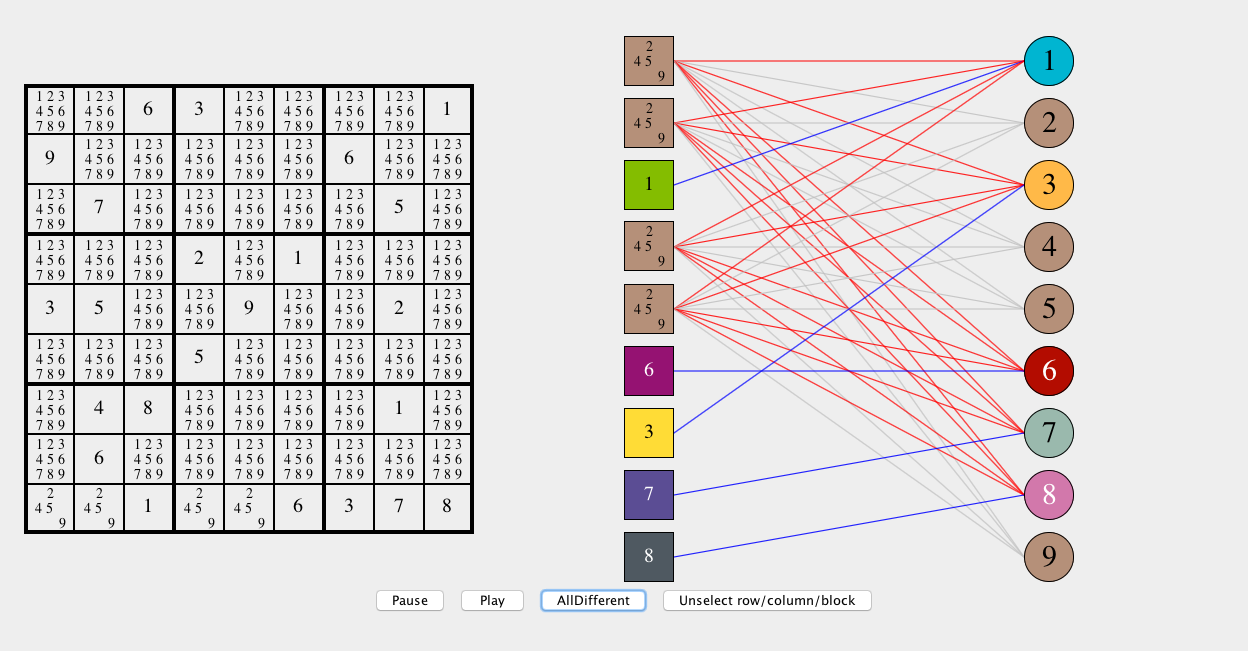
\includegraphics[width=13.2cm]{screenshot.png}
\caption{The state of the program after the all-different algorithm finishes on a row, in this case, the last one.}
\end{figure}


%==============================================================================

\chapter{Design and Implementation}
\label{design}

\section{High-Level Overview}
Model-View-Controller

\subsection{Problem Instance Representation}
Sudoku files

\section{Ford–Fulkerson's algorithm for computing a maximum matching}

\subsubsection{Origins}

\subsubsection{Description}

\subsubsection{Implementation}

\subsubsection{Visualisation}

\subsubsection{Discussion}

\section{Tarjan's algorithm for finding strongly connected components}

\subsubsection{Origins}

\subsubsection{Description}

\subsubsection{Implementation}

\subsubsection{Visualisation}

\subsubsection{Discussion}

Having a maximum matching for our graph, the next step in the alldifferent algorithm is to turn the previously undirected graph, into a directed one. The matches resulted from the Ford Fulkerson algorithm are assigned a direction from the 1 to 9 values to the corresponding cells of the Sudoku row. The edges that remain unused in the matching are given a direction from left to right (i.e. from the Sudoku cells of the row to the 1-9 values).

// write that we delete S/T nodes and corresponding edges

Now that all the edges from the graph are directed, the next step in the alldifferent algorithm is to find the strongly connected components of the graph. In order to do this, we introduce now Tarjan’s algorithm for finding strongly connected components  (SCCs) in a given graph G.

The algorithm starts by visiting every node in the directed graph in a depth first search manner. During the search, nodes are added to a stack in the order they are discovered only if they were not already part of the stack. 

Backtracking is triggered when we reach a node that is upper compared to our previous node (if(min < low[u])).  We know this by keeping record of the upmost node reachable from node u, including node u itself during each branch of the depth first search. We use low to denote the minimum index representing the upmost node in the branch.

If the current node is less than the upper node is less than the current index, it means that we have 

If the upper node is equal to the node we are currently visiting, then the algorithm just found a strongly connected component that contains all nodes on the stack starting from the top of it, until encountering the current node. The nodes are popped out of the stack and a SCC id/index is assigned to it for later use. Once the current node is reached, we increment the count of the SCCs to start filling a new SCC.

// write that there are no self loops / self edges (u!=i)
\cite{tarjan1972depth}

\begin{algorithm}
\DontPrintSemicolon
\nl $\textbf{void} ~Tarjan(\textbf{integer}~A[][],\textbf{int} ~ n)$ \;
\nl \Begin{
\nl $\textbf{Global} ~ S \gets ~new~\textbf{Stack}()$ \;
\nl $\textbf{Global} ~ stacked \gets ~new~\textbf{boolean}[n]$ \;
\nl $ $ \;
\nl $\textbf{Global} ~ pre \gets 0 $ \;
\nl $\textbf{Global} ~ count \gets 0 $ \;
\nl $ $ \;
\nl $\textbf{Global} ~ id \gets ~new~\textbf{integer}[n]$ \;
\nl $\textbf{Global} ~ low \gets ~new~\textbf{integer}[n]$ \;
\nl $ $ \;
\nl \For {$v \gets ~ 0 ~ to ~ n $}{
\nl \lIf {$stacked[v] = ~ false $}{ $dfs(v) $ }
}
}
\;
\nl $\textbf{void} ~dfs(\textbf{integer}~u)$ \;
\nl \Begin{
\nl $stacked[u] \gets ~true $\;
\nl $ $ \;
\nl $low[u] \gets ~pre $ \;
\nl $pre \gets pre + 1$ \;
\nl $\textbf{integer} ~ min \gets low[u] $ \;
\nl $ $ \;
\nl $push(S,u) $ \;
\nl $ $ \;
\nl \For {$i \gets ~ 0 ~ to~ A[u].length$}{
\nl $\textbf{integer} ~ w \gets A[u][i] $ \;
\nl $ $ \;
\nl \If {$w = 1 ~\bf{and} ~ u \neq i$}{
\nl \lIf {$stacked[i] = ~false $}{ $dfs(~i) $ }
\nl \lIf {$low[i] < min $}{ $ min \gets low[i] $ }
  }
 }
\nl $ $ \;
\nl \If {$ min < low[u] $}{
\nl $low[u] \gets min $ \;
\nl $\textbf{return} $ \;
}
\nl $ $ \;
\nl $\textbf{integer} ~ w $ \;
\nl $ $ \;
\nl \Repeat{\nl $w \neq u$}{
\nl $w \gets pop(S) $ \;
\nl $id[w] \gets count $ \;
\nl $low[w] \gets n $ \;
 }
\nl $ $ \;
\nl $ count \gets count + 1 $ \;

}
\caption{Tarjan's strongly connected components}
\label{TarjanPC}
\end{algorithm}

%\lstset{language=Java}

%\begin{figure}
%\lstset{caption={Implementation of Tarjan's algorithm %for finding strongly connected %components},label=codeTarjan}
%\lstinputlisting{Tarjan.java}
%\end{figure}

\chapter{Conclusion}
\label{conclusion}
We have shown how to implement the all-different constraint.

%%%%%%%%%%%%%%%%
%              %
%  APPENDICES  %
%              %
%%%%%%%%%%%%%%%%
\begin{appendices}

\chapter{Running the Program}
An example of running from the command line is as follows:
\begin{verbatim}
      > javac *.java
      > java Sudoku
\end{verbatim}
This will open the application loaded with the hard Sudoku problem $/herald20061222H.txt$.

\noindent
\textbf{TODO}: what about the Choco3 library? add it to path? remove it?

\chapter{Proof of concept}

The following sequence of steps will provide a visual proof of the all-different algorithm. The following figures capture the user running the all-different algorithm on 5 predetermined rows, columns or 3x3 sub-grids. For demonstration purposes, the Sudoku instance used is $lockedset.txt$.

The sequence is as follows:
\begin{verbatim}
      > Open lockedset.txt Sudoku instance
      >
      > Select the 1st column
      > Run the all-different algorithm
      > Unselect
      >
      > Select the 5th row
      > Run the all-different algorithm
      > Unselect
      >
      > Select the 6th row
      > Run the all-different algorithm
      > Unselect
      >
      > Select the 4th 3x3 sub-grid
      > Run the all-different algorithm
      > Unselect
      >
      > Select the 1st column
      > Run the all-different algorithm
      > Unselect
\end{verbatim}

Alternatively, the user can press the $Show Demo$ button to run the same steps.

\begin{figure}[h]
\hfill
\subfigure[1st column after running the all-different algorithm]{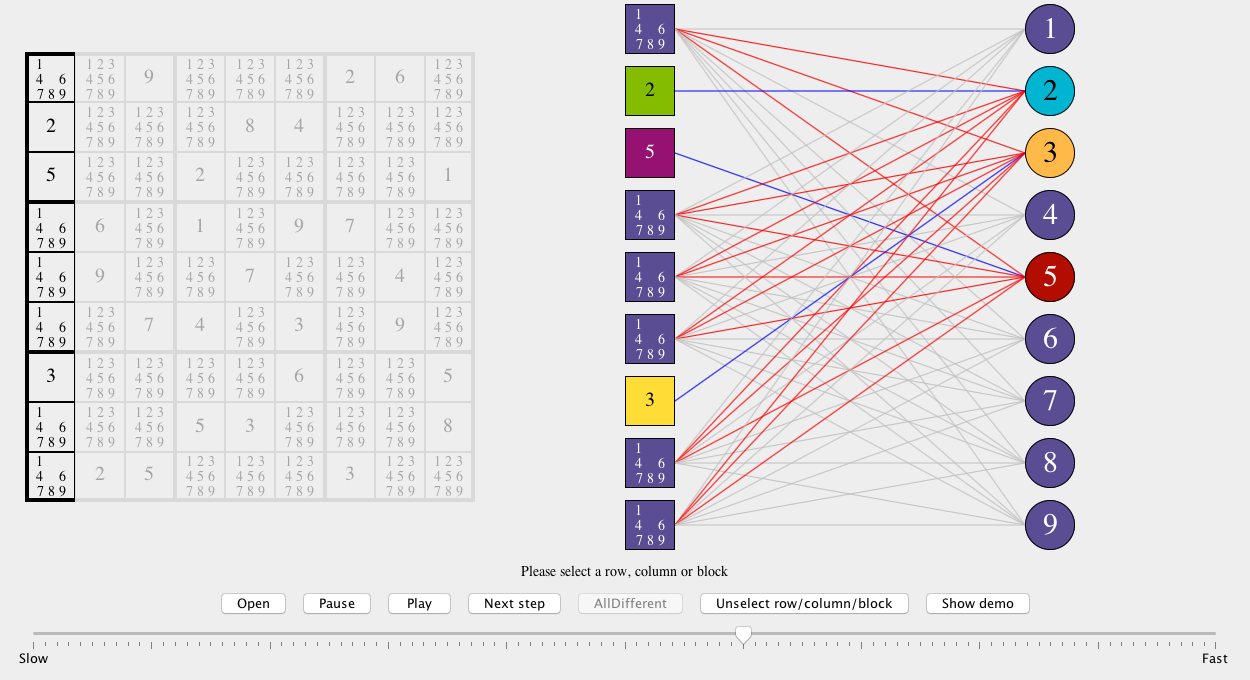
\includegraphics[width=8cm]{images/proof_of_concept/1.png}}
\hfill
\subfigure[5th row after running the all-different algorithm]{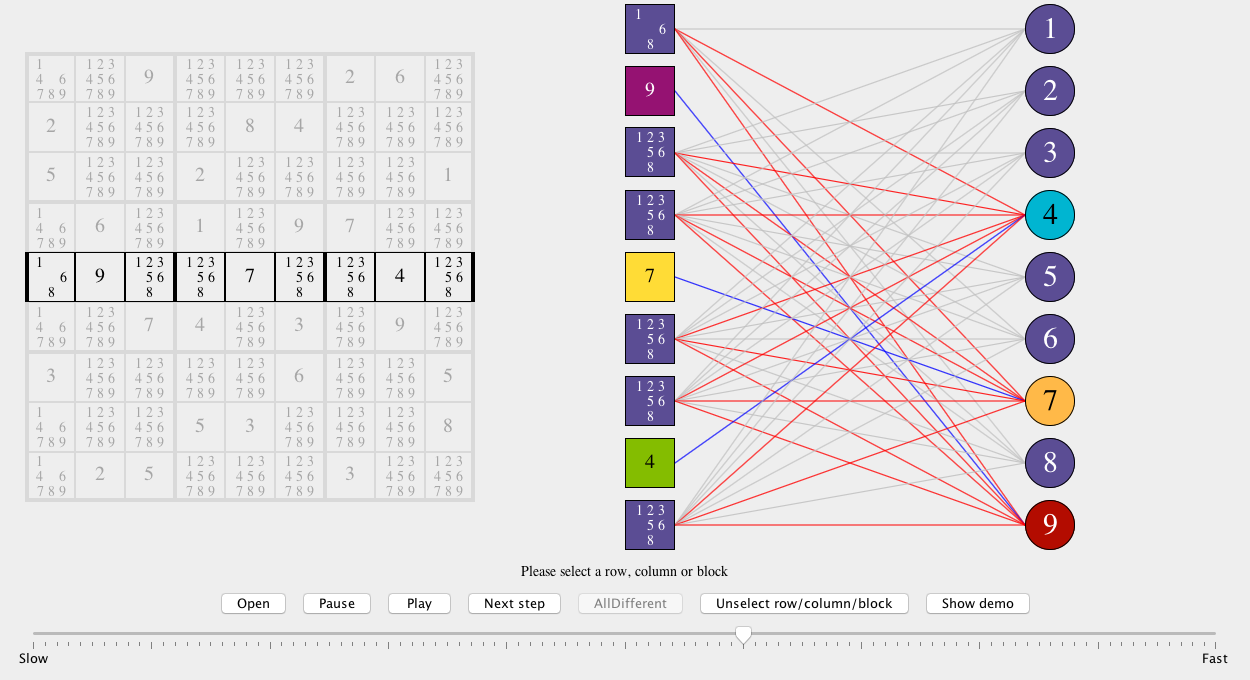
\includegraphics[width=8cm]{images/proof_of_concept/2.png}}
\vspace*{2cm}
\hfill
%\caption{Title for both}
%\end{figure}

%\begin{figure}[h]
\hfill
\subfigure[6th row after running the all-different algorithm]{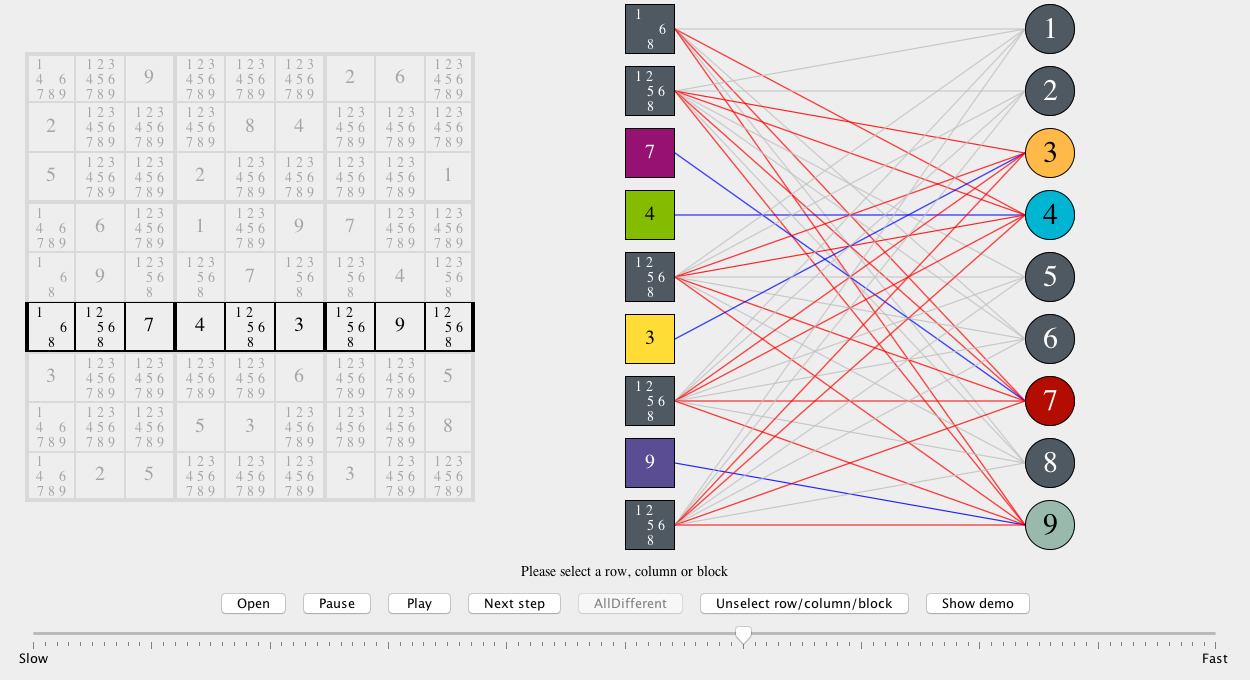
\includegraphics[width=8cm]{images/proof_of_concept/3.png}}
\hfill
\subfigure[4th 3x3 sub-grid after running the all-different algorithm]{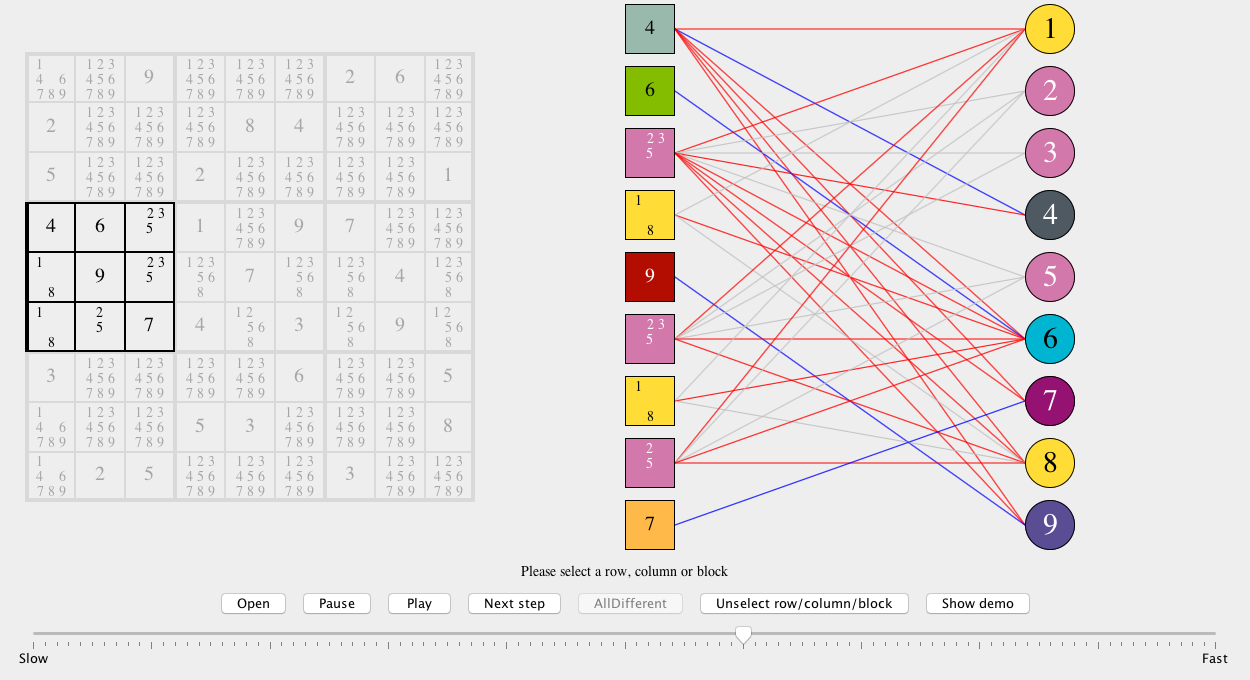
\includegraphics[width=8cm]{images/proof_of_concept/4.png}}
\vspace*{2cm}
\hfill
%\caption{Title for both}
%\end{figure}

%\begin{figure}[h]
\hfill
\subfigure[1st column after running the all-different algorithm]{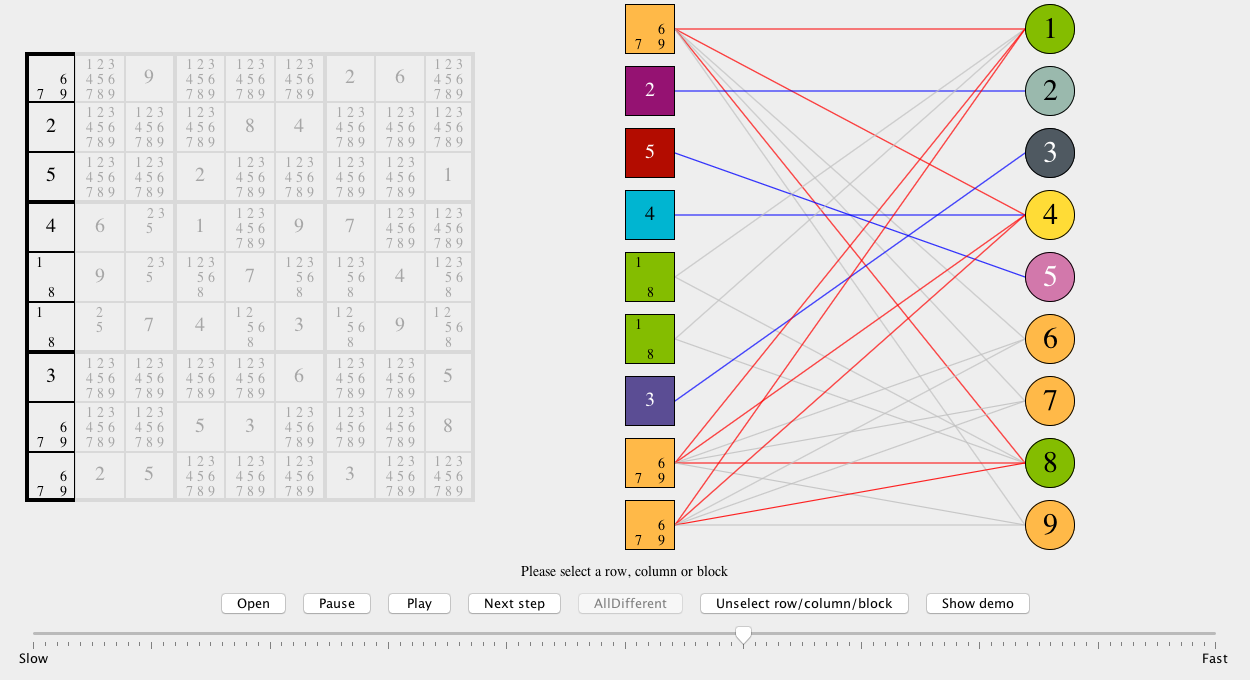
\includegraphics[width=8cm]{images/proof_of_concept/5.png}}
\hfill
%\subfigure[Proof]{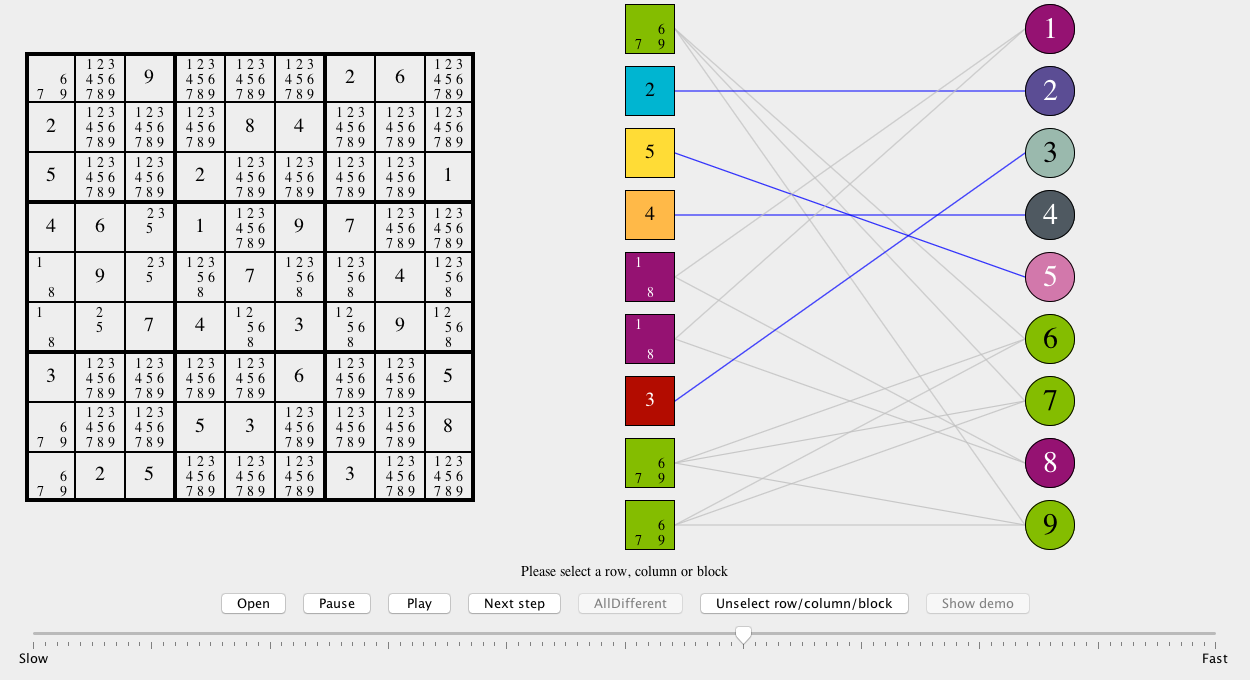
\includegraphics[width=8cm]{images/proof_of_concept/6.png}}
\hfill
\caption{Steps in the demo}
\label{fig:proof_1_5}
\end{figure}

\clearpage 

\begin{figure}[h]
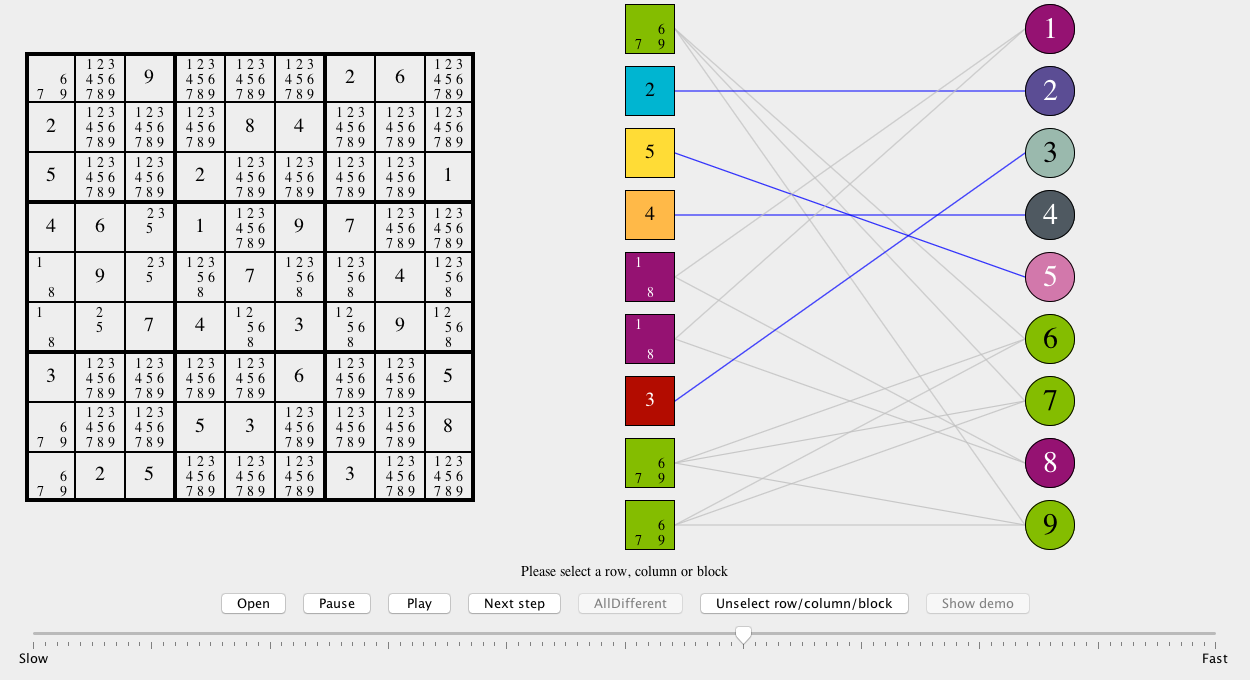
\includegraphics[width=16cm]{images/proof_of_concept/6.png}
\caption{State of the program after running the demo}
\label{fig:proof_6}
\end{figure}

As seen in ~\Cref{fig:proof_1_5}, the all-different algorithm performs changes only to the selected 9 cells  inside a row, column or 3x3 sub-grid. 

The end result of following the above steps can be seen in ~\Cref{fig:proof_6}. This state mimics the human thinking when solving a Sudoku. In the 1st column there are two cells with a domain of ${1, 8}$, but we don't know yet which cell will take which digit. What we do know though, is that the digits ${1, 8}$ will be distributed in that two particular cells, therefore in the last step, after running the all-different algorithm on the 1st column we can observe that the digits ${1, 8}$ disappear from the domains of the rest of the cells in the selection.

\end{appendices}

%%%%%%%%%%%%%%%%%%%%
%   BIBLIOGRAPHY   %
%%%%%%%%%%%%%%%%%%%%

\bibliographystyle{plain}
\bibliography{bib}

\end{document}
